\documentclass[ngerman]{dis-template-add}


\renewcommand{\Aufgabenblatt}{5}
\renewcommand{\Ausgabedatum}{9. Juni 2020}
\renewcommand{\Abgabedatum}{23. Juni 2020}
\renewcommand{\Gruppe}{Simon Weidmann, Aram Yesildeniz}
\renewcommand{\STiNEGruppe}{14}


\begin{document}


\section*{5.1 Tutorial}

\subsection*{Insert}

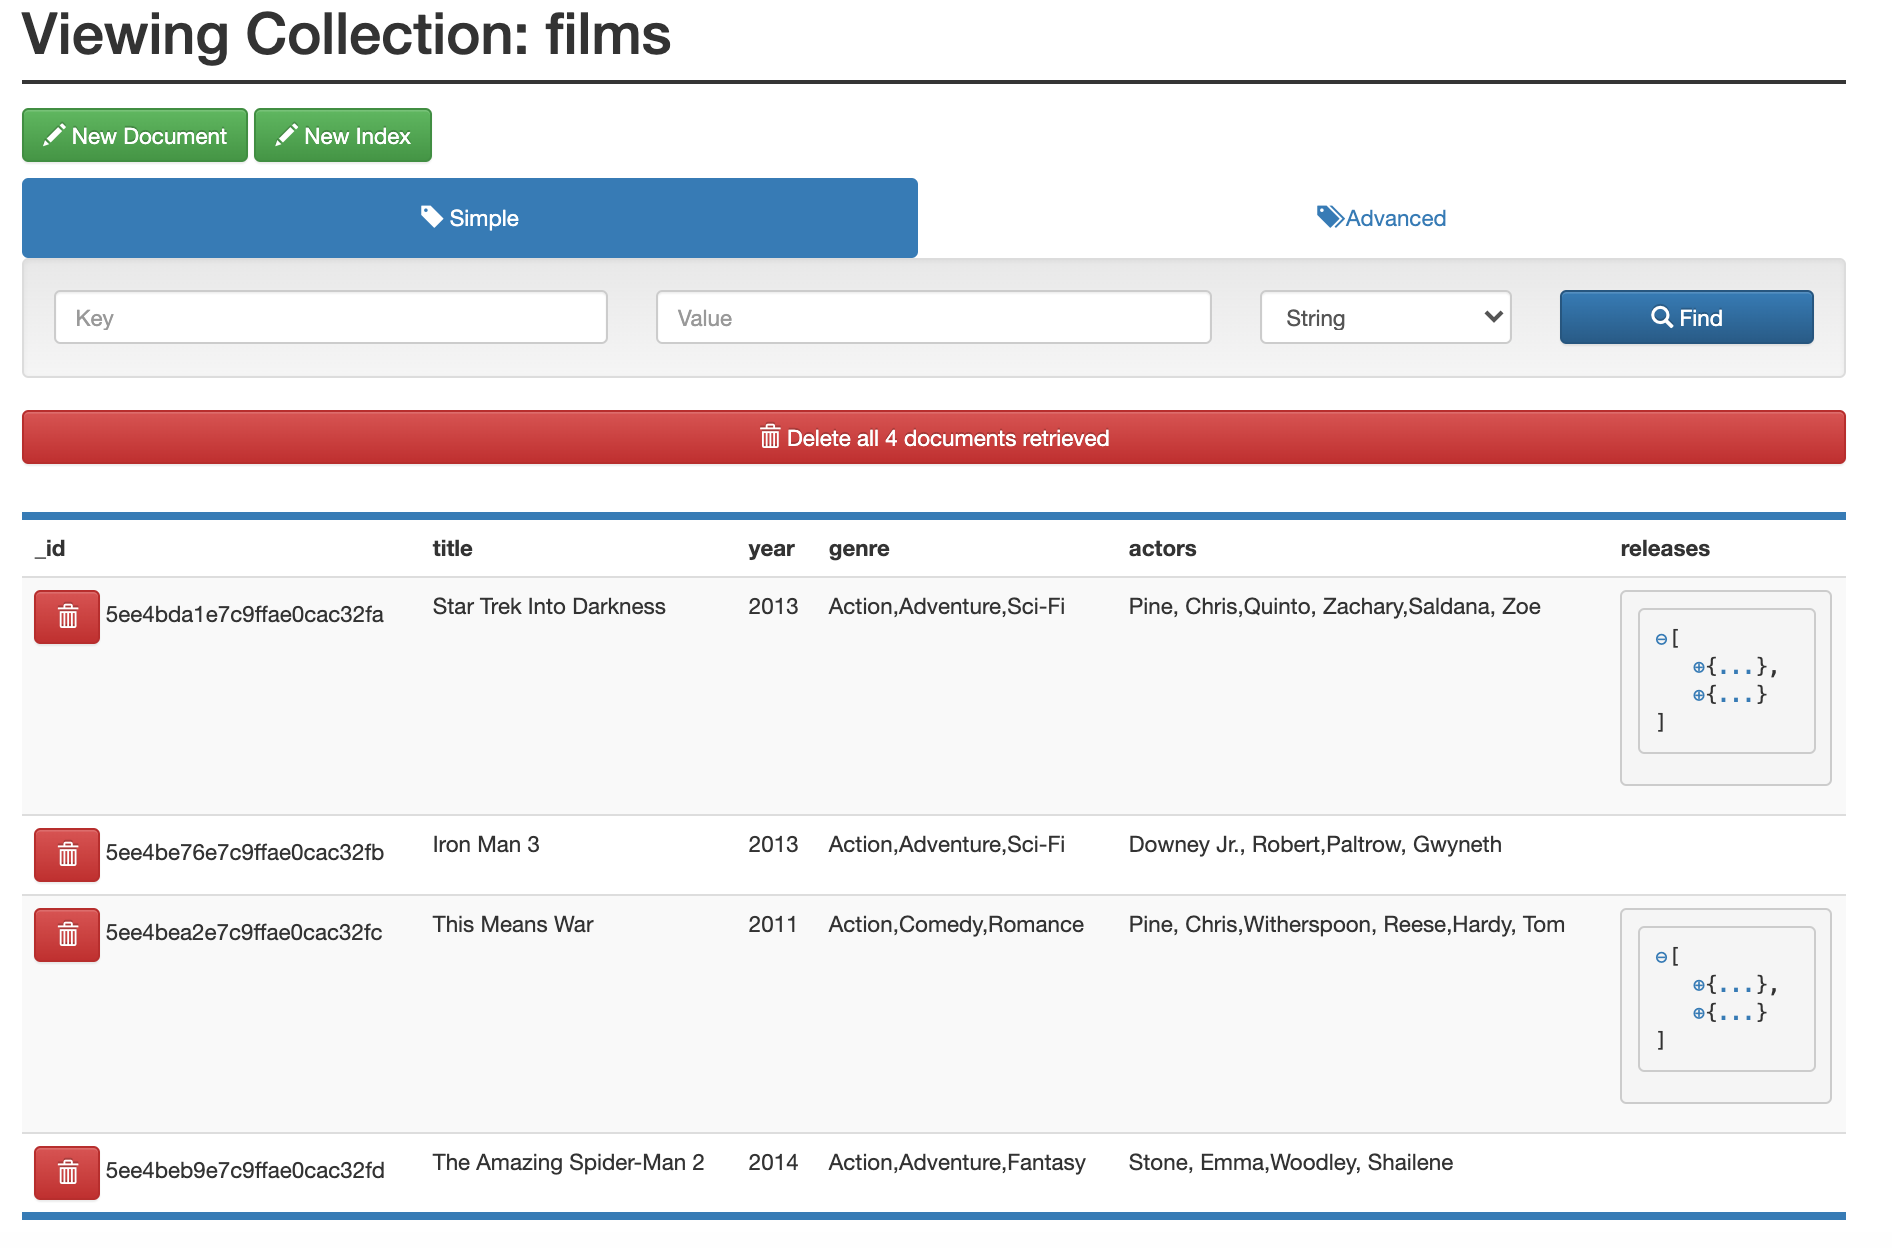
\includegraphics[scale=0.3]{insert.png}

\subsection*{Querying}

Example of one query:

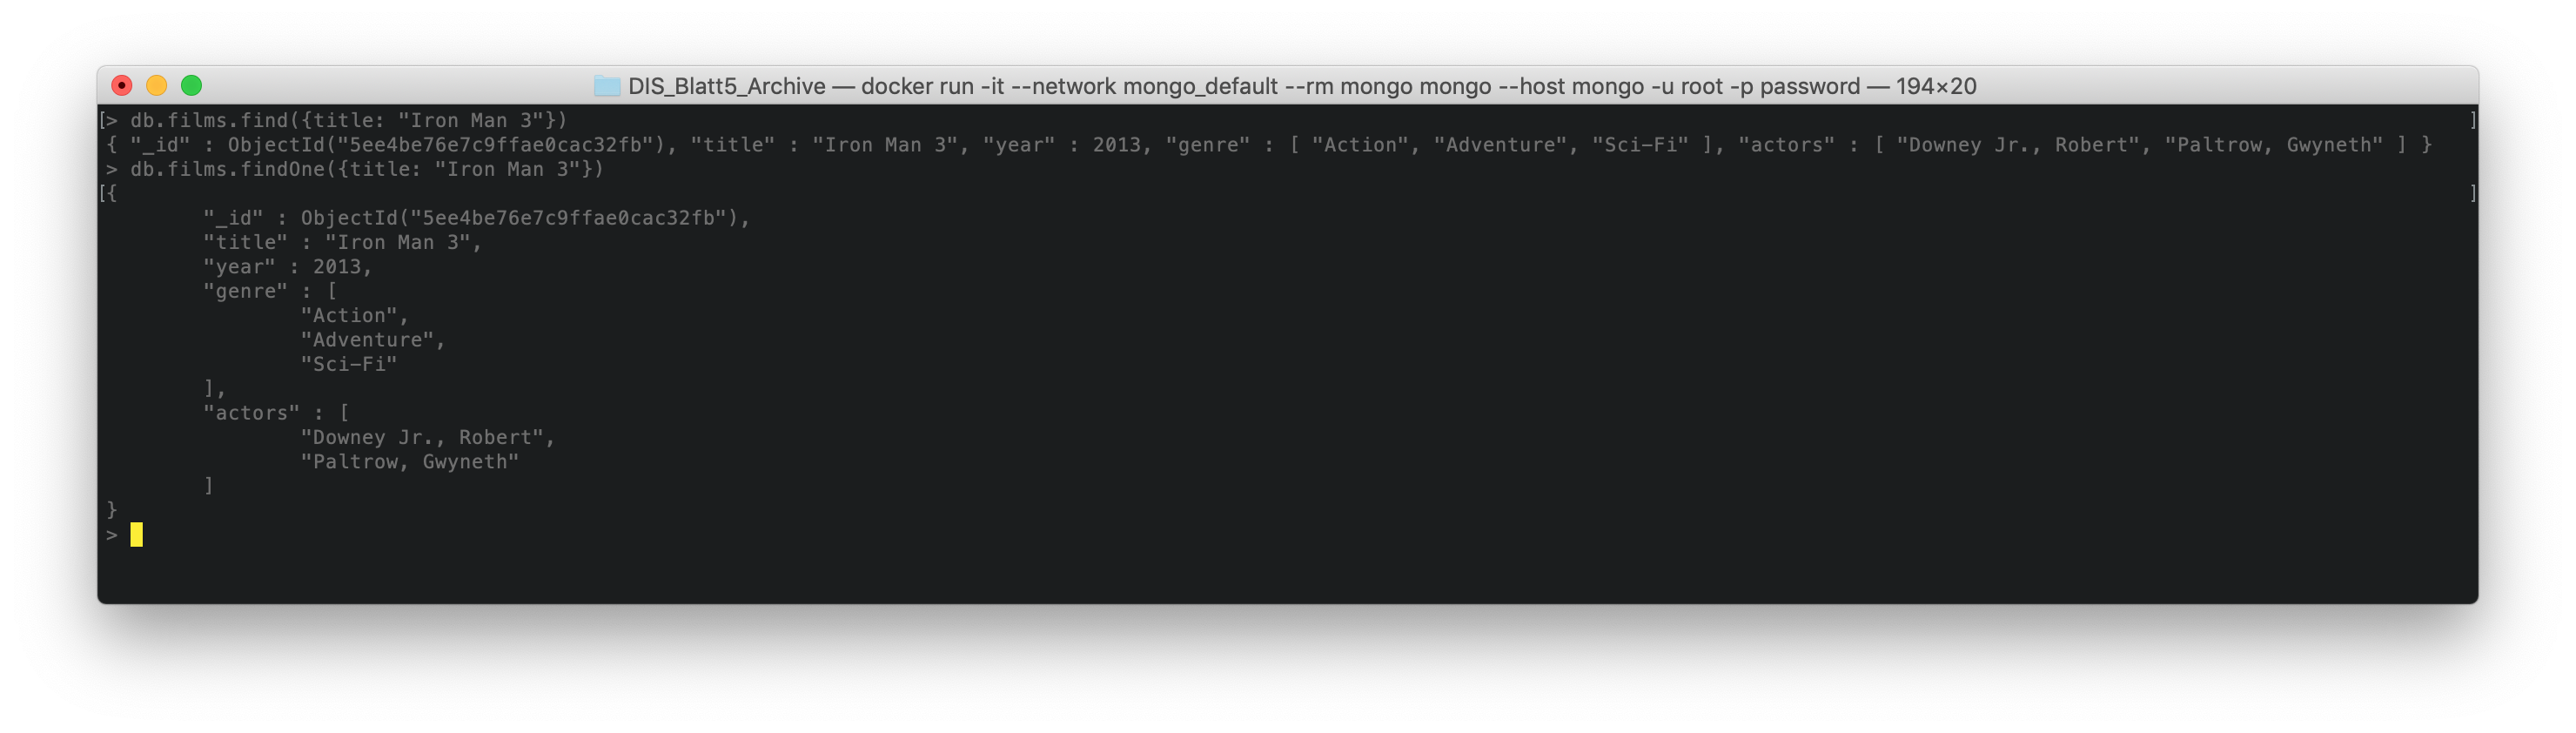
\includegraphics[scale=0.3]{query.png}

\subsection*{Update}

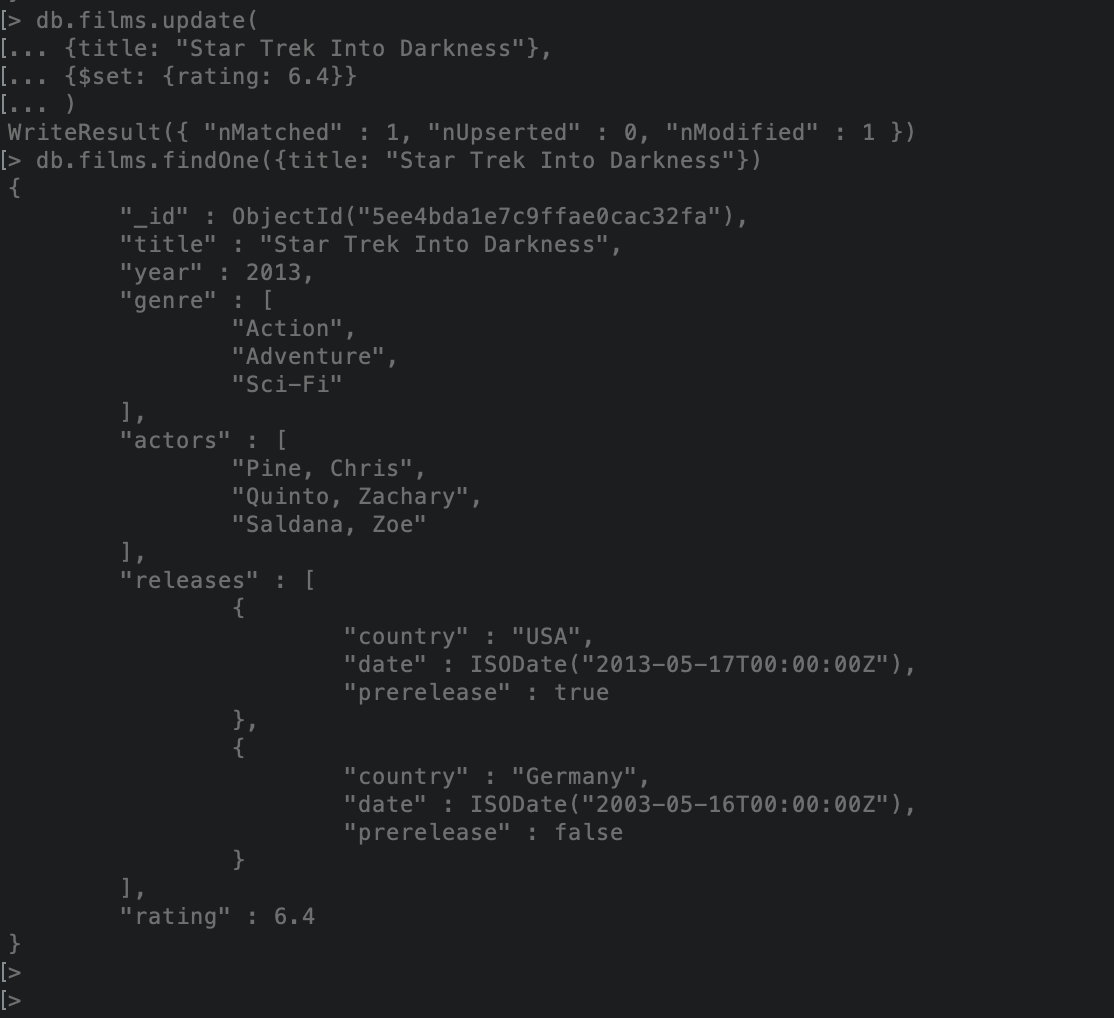
\includegraphics[scale=0.3]{update.png}

\subsection*{Delete}

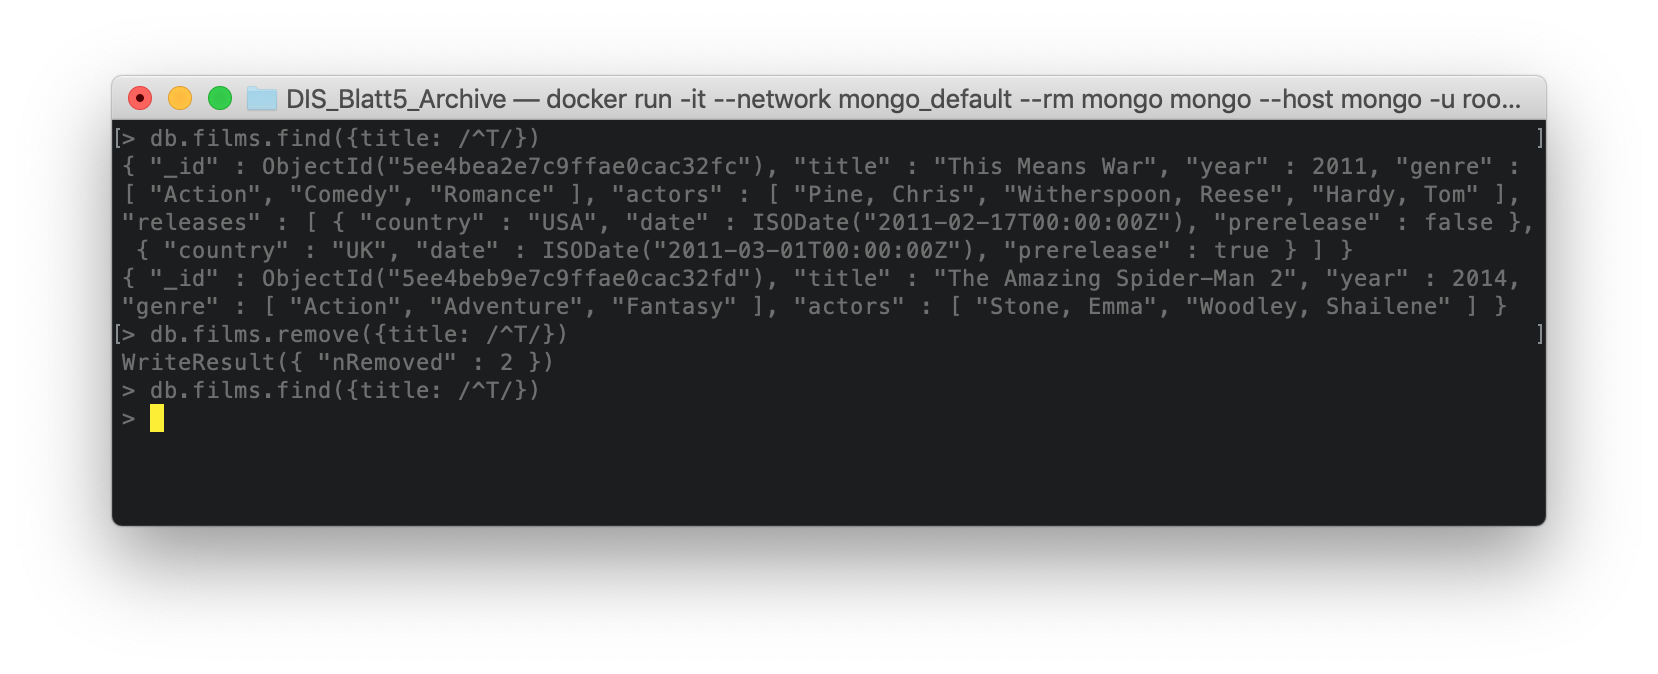
\includegraphics[scale=0.3]{delete.png}

\subsection*{Indexing}

Without index: 
\begin{verbatim}
"executionTimeMillis" : 202
\end{verbatim}

With index:
\begin{verbatim}
"executionTimeMillis" : 165
\end{verbatim}



\section*{5.2 Movie mApp}

The following screenshots are showing the results of different queries and usage of the Movie mApp. Please consider the source code for implementation details.

\subsection*{Search Movie}
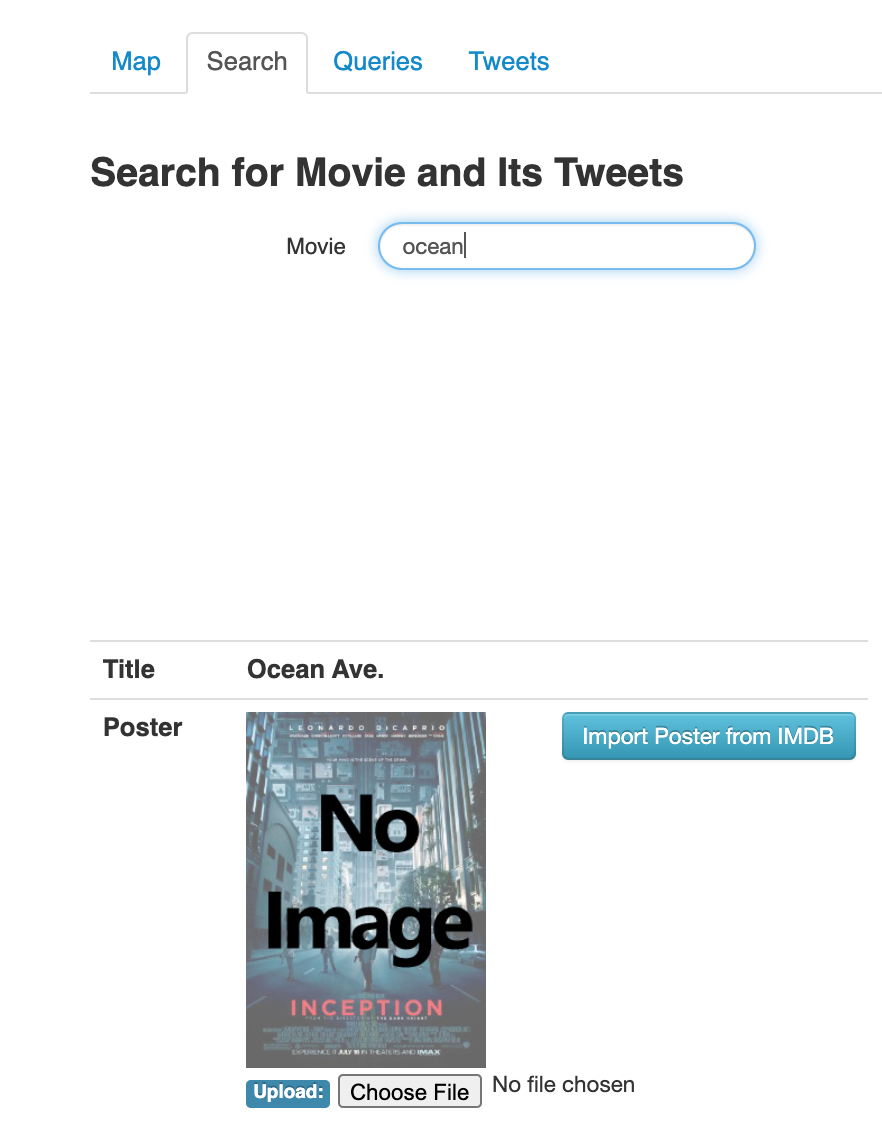
\includegraphics[scale=0.3]{1-movie_search.png}

\subsection*{Load Poster}
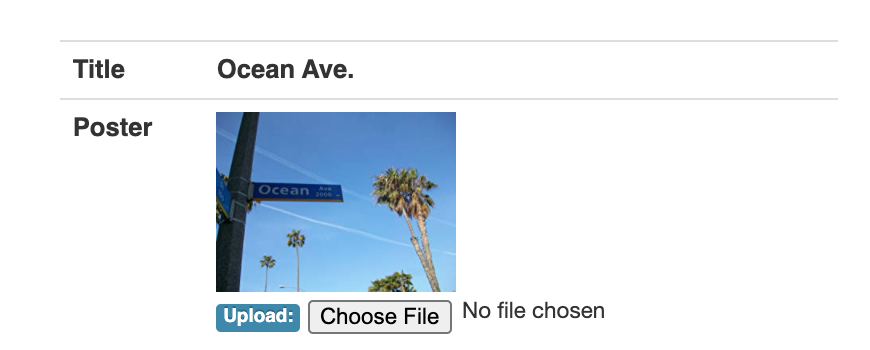
\includegraphics[scale=0.3]{2-load_image.png}

\subsection*{Change Comment}
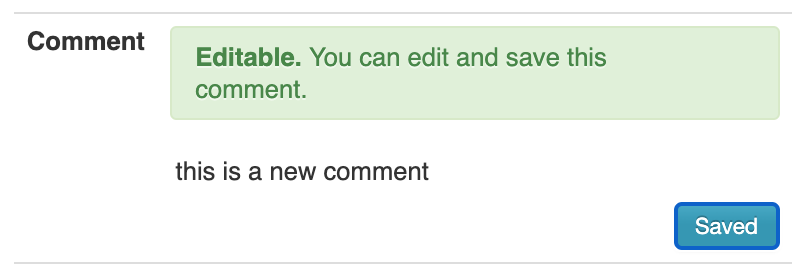
\includegraphics[scale=0.3]{3-change_comment.png}

\subsection*{Rating}
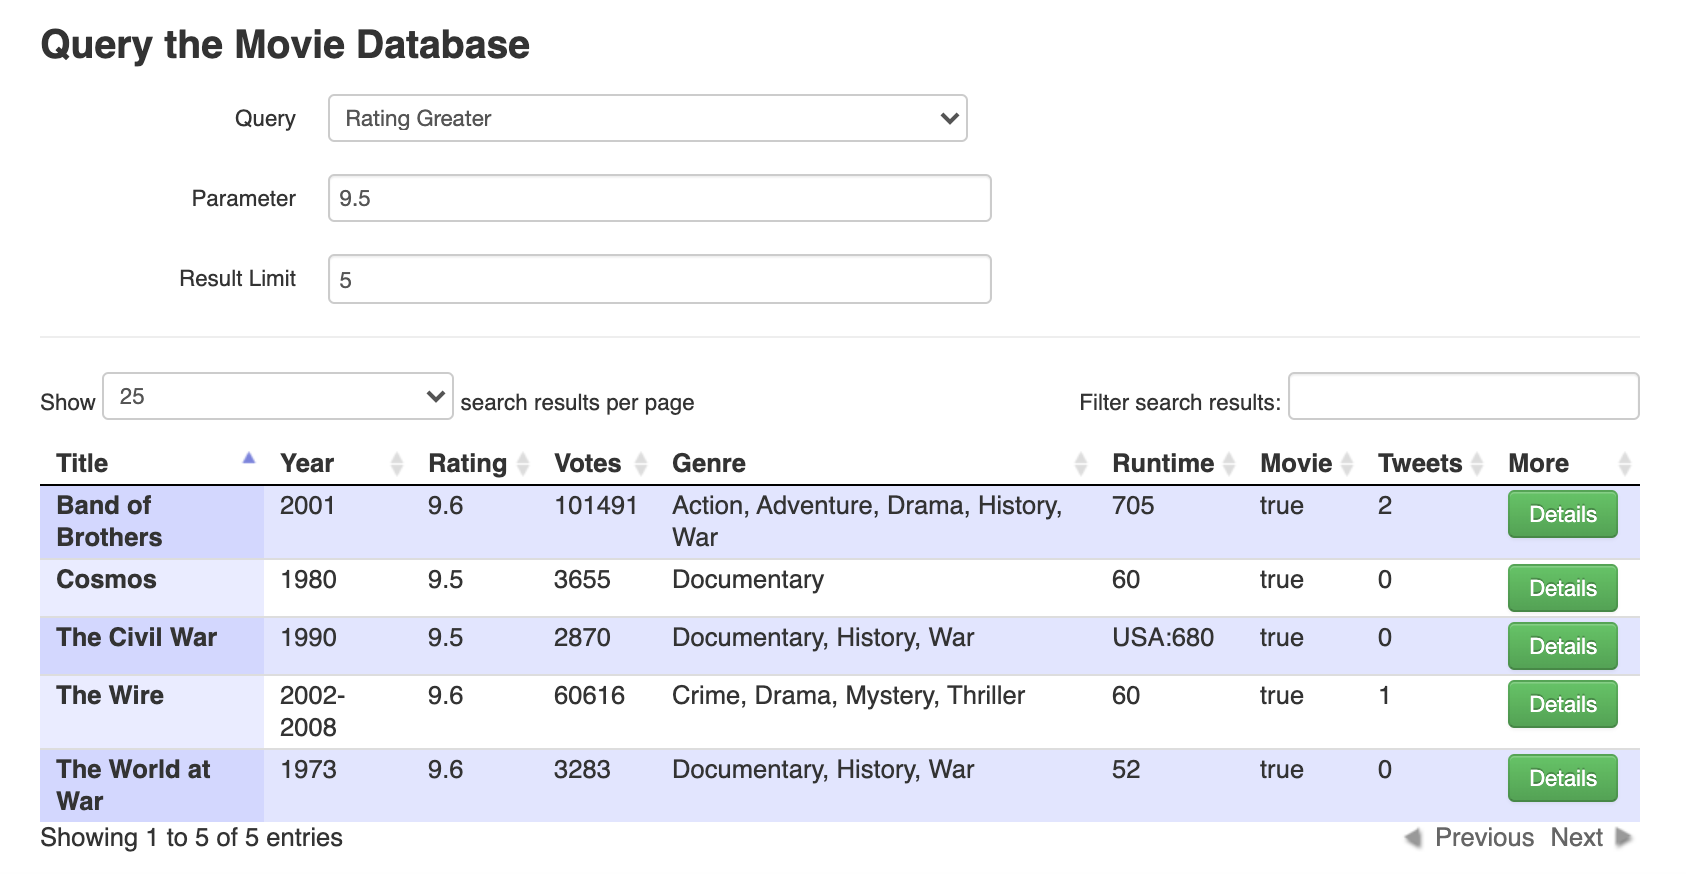
\includegraphics[scale=0.3]{4-rating.png}

\subsection*{Search Title Prefix}
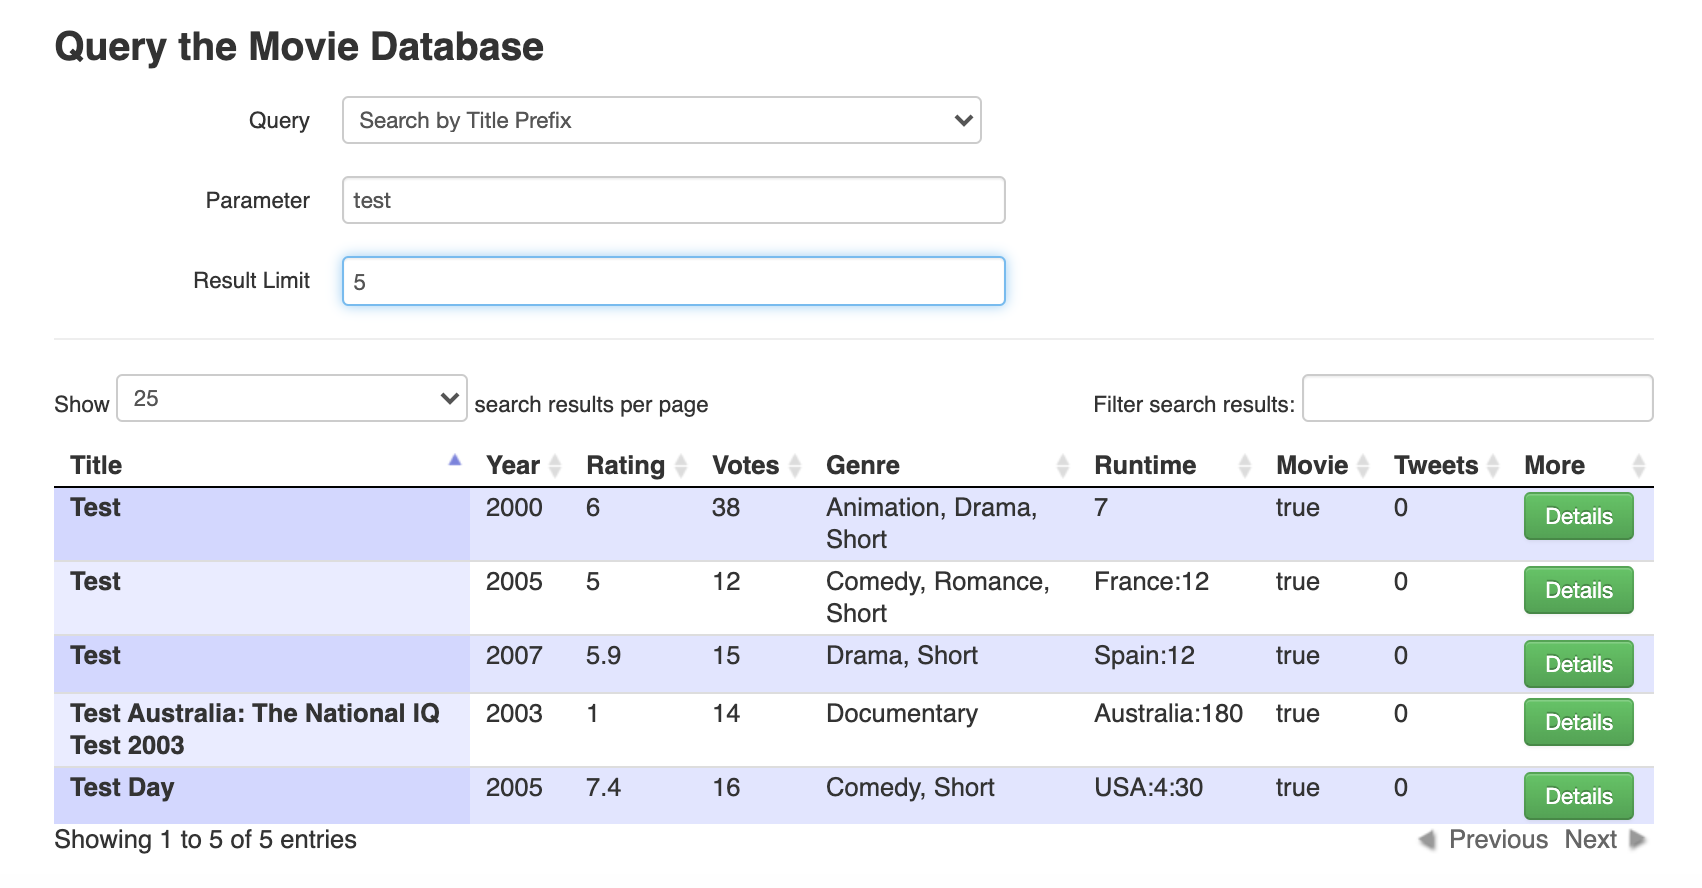
\includegraphics[scale=0.3]{5-title_prefix.png}

\subsection*{Tweet Keyword}
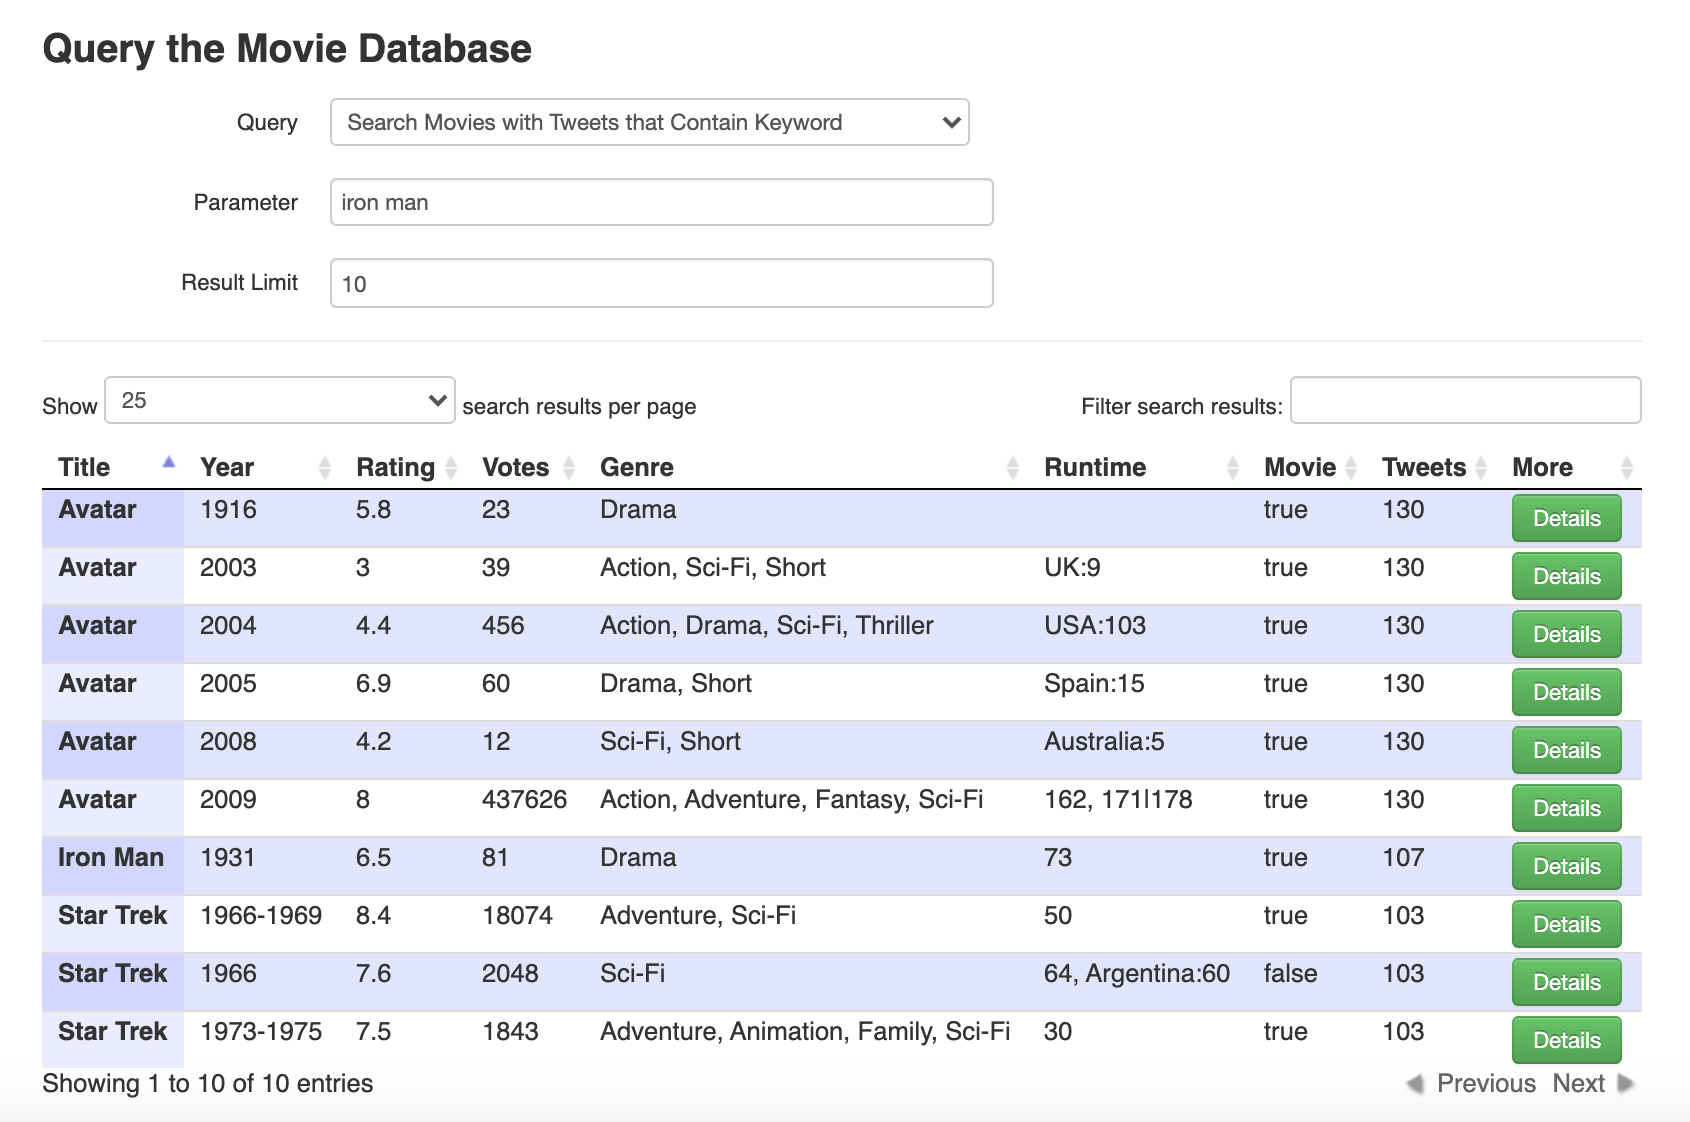
\includegraphics[scale=0.3]{6-tweet_keyword.png}

\subsection*{Search by Genre}
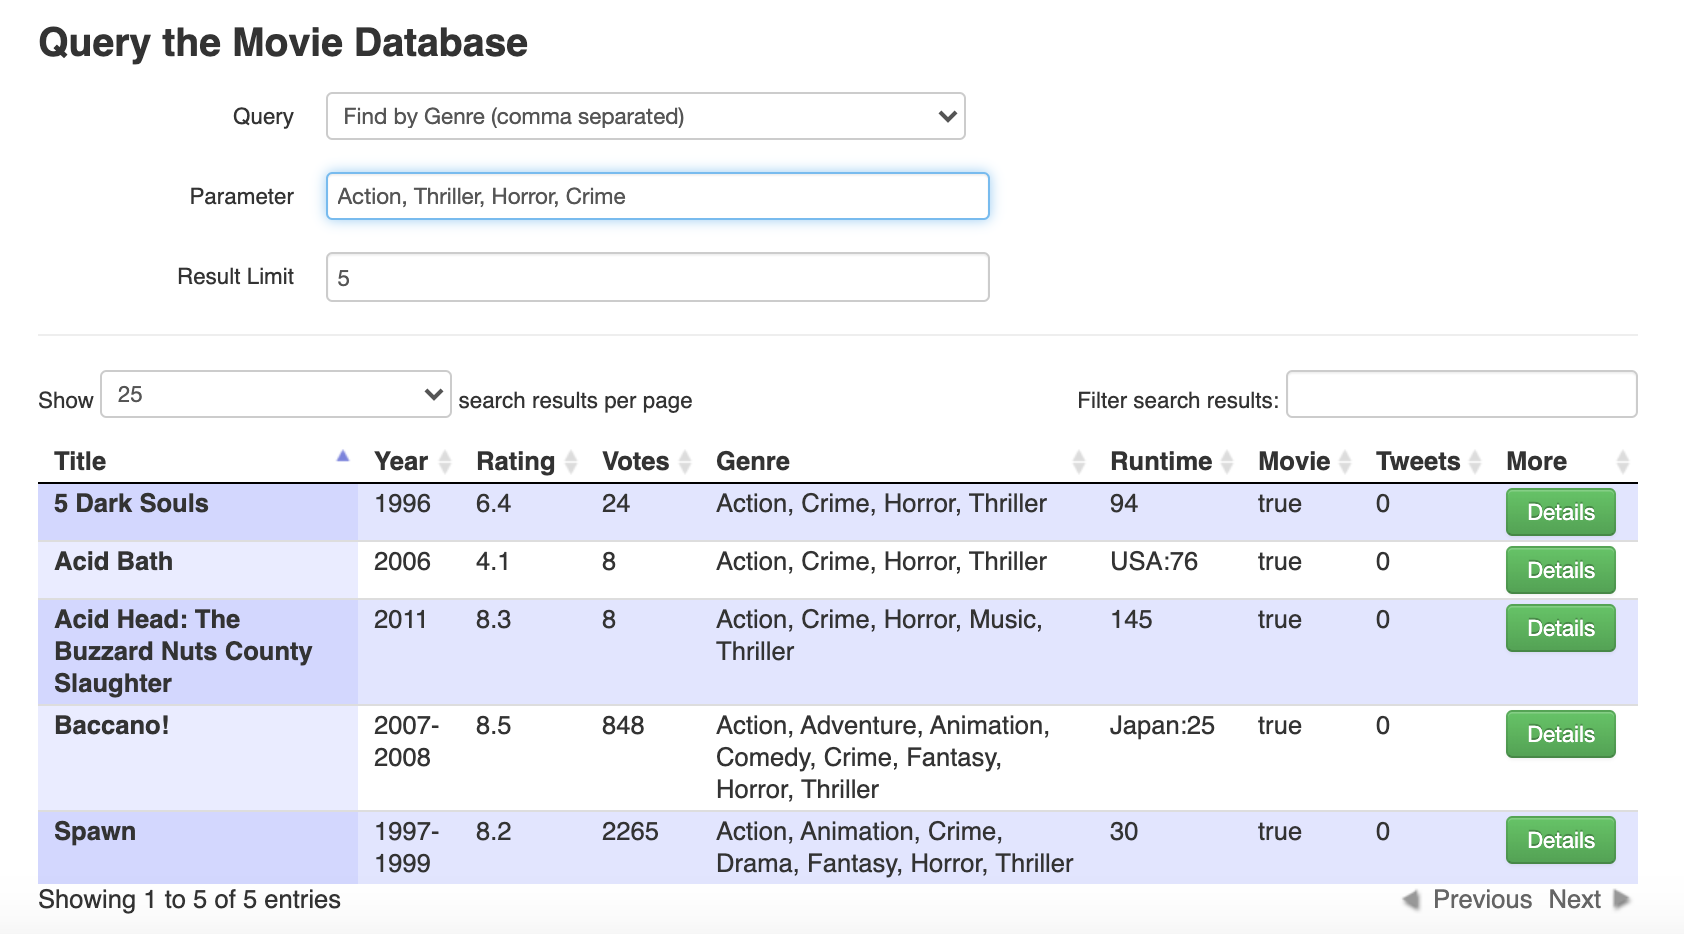
\includegraphics[scale=0.3]{7-genre.png}

\subsection*{Movie Tweets}
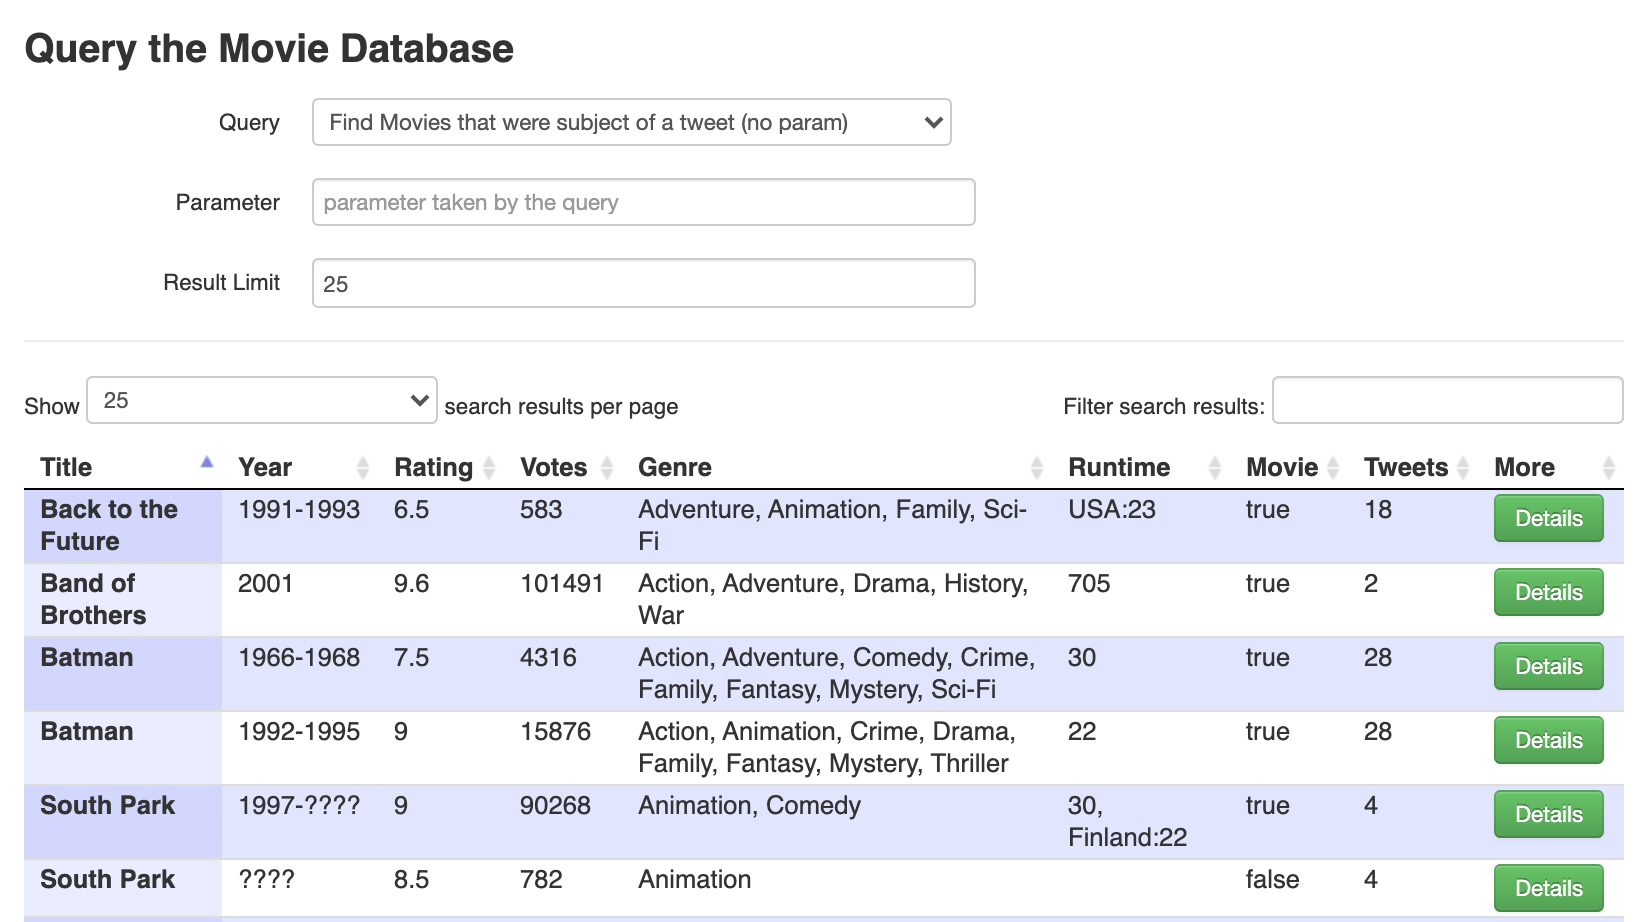
\includegraphics[scale=0.3]{8-movie_tweet.png}

\subsection*{FTS}
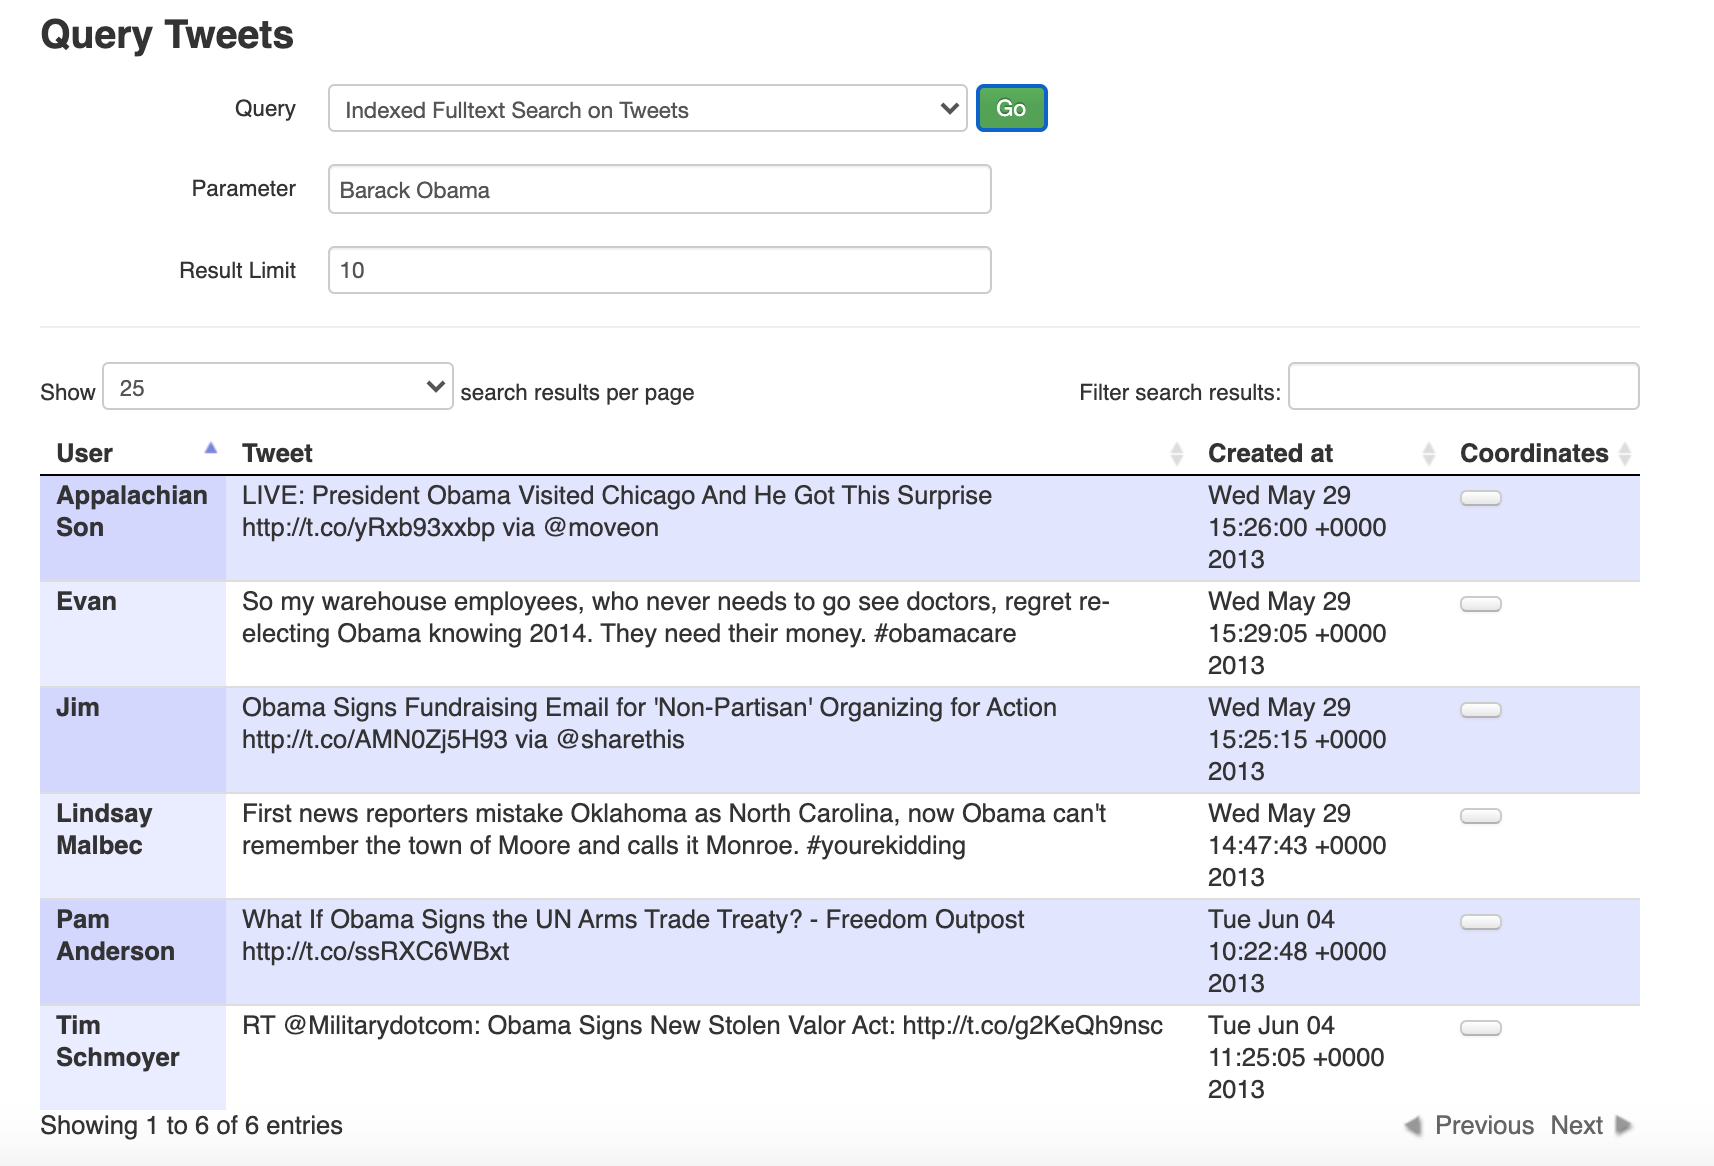
\includegraphics[scale=0.3]{9-fts.png}

\subsection*{Newest Tweets}
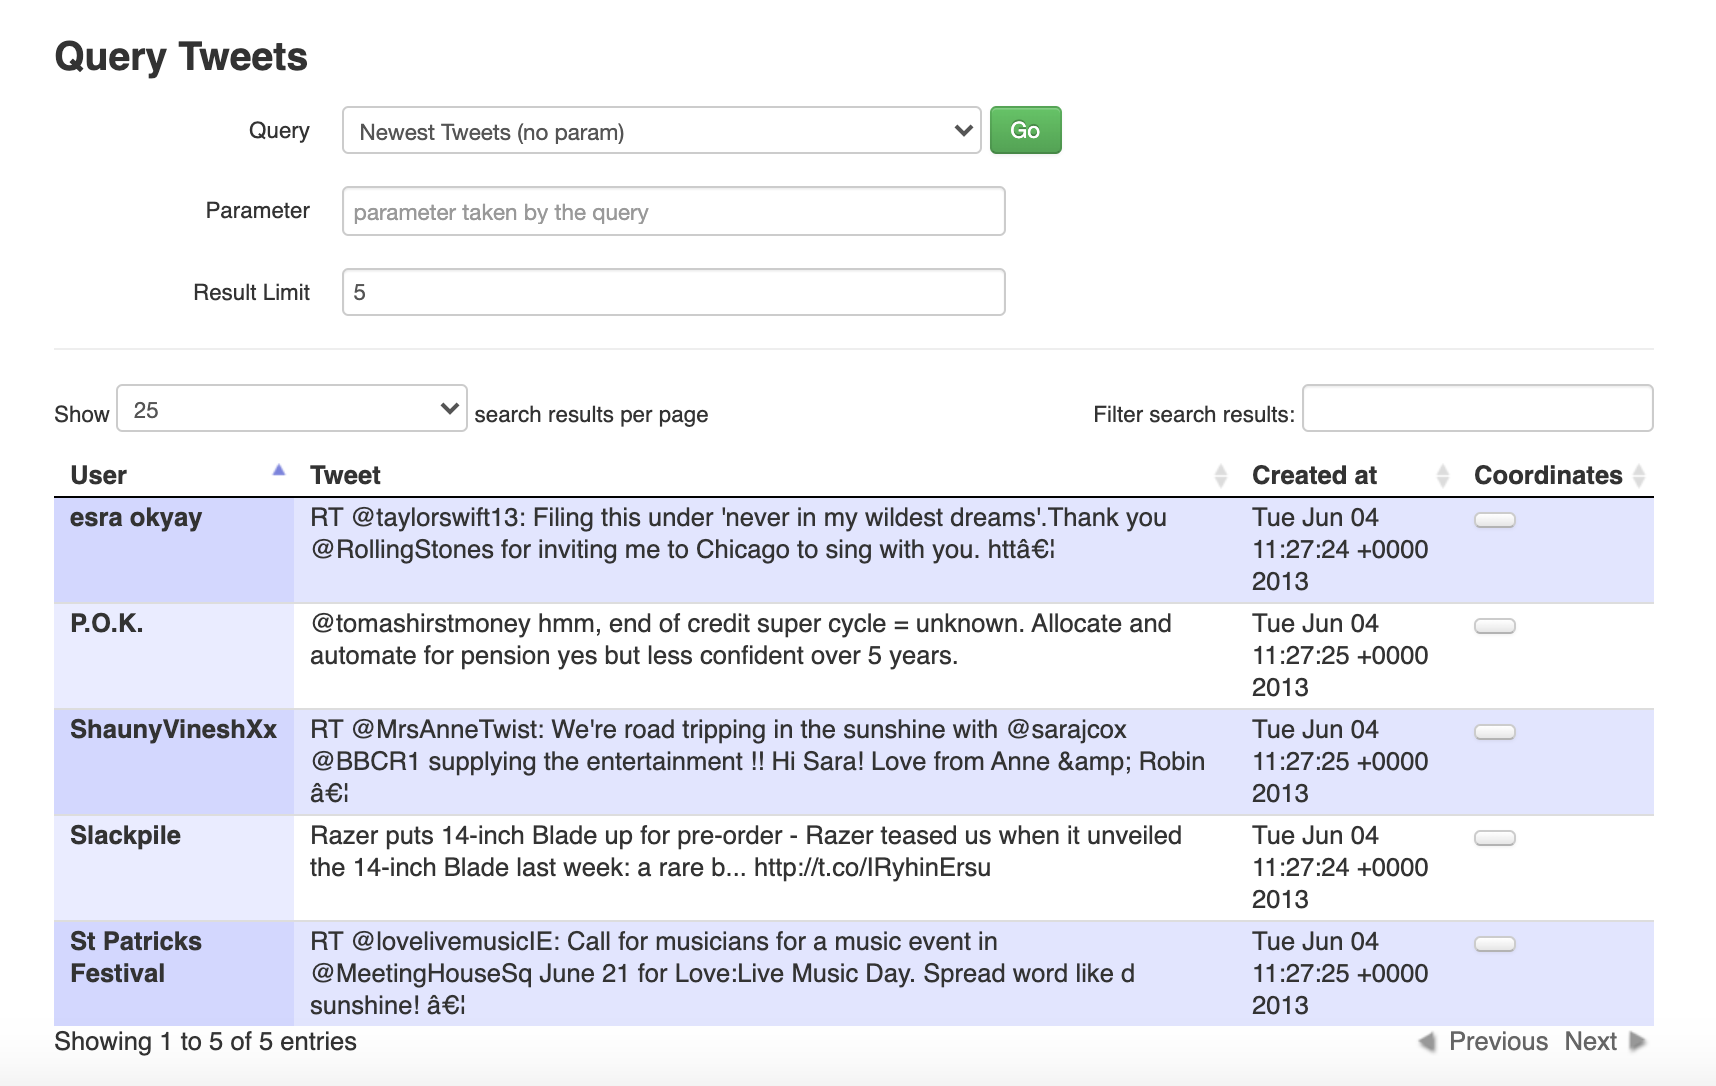
\includegraphics[scale=0.3]{10-newest_tweet.png}


\end{document}